% !TEX root = task-1-12-3.tex
% Editable task bank. Append new BankTask blocks at the end of the document.
\documentclass[12pt,a4paper]{article}
\usepackage{physics-textbook}
\usepackage{graphicx,needspace}
\usetikzlibrary{decorations.pathmorphing}
\newif\ifShowSolutions
\ifdefined\TutorEdition
  \ShowSolutionstrue
\else
  \ShowSolutionsfalse % Change to \ShowSolutionstrue to display solutions.
\fi
\newcounter{banktask}
\newsavebox{\BankTaskBox}
\newcommand{\BankTaskContent}[3]{%
  \noindent\textbf{\thebanktask.}\quad #2\par
  \ifShowSolutions
    \Needspace{50mm}% Keep the solution heading with its opening text or diagram.
    #3\par
    \ifdefined\TutorEdition
      \ifcsname TutorSource#1\endcsname
        \nopagebreak\smallskip{\small\csname TutorSource#1\endcsname\par}%
      \fi
    \fi
  \fi
}
\newcommand{\BankTask}[3]{%
  \refstepcounter{banktask}\par\medskip
  \sbox{\BankTaskBox}{\begin{minipage}{\linewidth}%
    \BankTaskContent{#1}{#2}{#3}\end{minipage}}%
  \ifdim\dimexpr\ht\BankTaskBox+\dp\BankTaskBox\relax>\dimexpr\textheight-20mm\relax
    \Needspace{35mm}\BankTaskContent{#1}{#2}{#3}%
  \else
    \Needspace{\dimexpr\ht\BankTaskBox+\dp\BankTaskBox\relax}%
    \noindent\usebox{\BankTaskBox}\par
  \fi
  \medskip
}
\begin{document}
\BookSubsection{1.12.3}{Центр масс и центр тяжести}


% Source 25401: https://phys-ege.sdamgia.ru/problem?id=25401
\BankTask{25401}{
Деревянная линейка длиной l  =  $90\,\text{см}$ выдвинута за край стола на $\frac{1}{4}$ часть своей длины. При этом она не опрокидывается, если на ее правом конце лежит груз массой не более $m_1=250\,\text{г}.$ Далее линейку выдвинули вправо за край стола на некоторое расстояние и положили на ее правый конец груз массой $m_2=125\,\text{г}.$ На какое расстояние дополнительно можно выдвинуть линейку во втором опыте, чтобы она не перевернулась?
}{
\smallskip\noindent\textbf{Решение}\par
На линейку в обоих случаях действую сила тяжести линейки, приложенная к ее середине и вес груза. Линейка находится в равновесии, поэтому можно записать правило моментов для каждого случая относительно точки опоры  — края стола. В первом случае плечи силы тяжести линейки и веса груза равны $\frac{l}{4} .$ 
Следовательно, масса линейки равна массе груза $M=m_1=250\,\text{г}.$

\begin{center}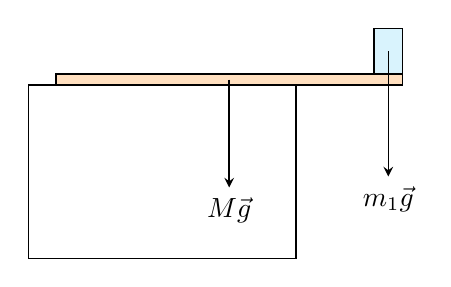
\begin{tikzpicture}[>=stealth,line width=.55pt]\draw(0,-2.2)rectangle(3.4,0);\draw[fill=orange!25](.35,0)rectangle(4.75,.14);\draw[fill=cyan!15](4.39,.14)rectangle(4.75,.72);\draw[->](4.57,.43)--(4.57,-1.16)node[below]{$m_1\vec g$};\draw[->](2.55,.07)--(2.55,-1.3)node[below]{$M\vec g$};\end{tikzpicture}\end{center}

\begin{center}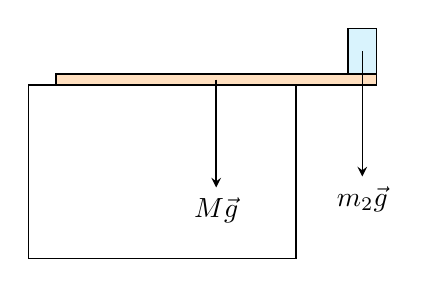
\begin{tikzpicture}[>=stealth,line width=.55pt]\draw(0,-2.2)rectangle(3.4,0);\draw[fill=orange!25](.35,0)rectangle(4.42,.14);\draw[fill=cyan!15](4.06,.14)rectangle(4.42,.72);\draw[->](4.24,.43)--(4.24,-1.16)node[below]{$m_2\vec g$};\draw[->](2.385,.07)--(2.385,-1.3)node[below]{$M\vec g$};\end{tikzpicture}\end{center}

Во втором случае плечо веса груза равно $l_2$ а плечо силы тяжести линейки $\frac{l}{2} - l_2.$
Запишем правило моментов для второго случая:

$m_2gl_2=Mg ( \frac{l}{2} - l_2 ) ,$ откуда плечо веса груза:
$l_2= \frac{Ml}{2 ( m_2 + M )} = \frac{250 \cdot 90}{2 \cdot ( 125 + 250 )} =30\,\text{см}.$

Учитывая, что в первом случае расстояние равнялось $\frac{l}{4} = \frac{90}{4} =22{,}5\,\text{см},$ линейка останется в равновесии, если ее выдвинуть на $7{,}5\,\text{см}$.

Ответ: $7{,}5\,\text{см}$.
}

% Source 42654: https://phys-ege.sdamgia.ru/problem?id=42654
\BankTask{42654}{
\begin{center}\begin{tikzpicture}[task graph,>=stealth]
\draw(-.3,0)--(3,0)--(3,-.8);
\foreach \x in {0,.2,...,2.8}{\draw(\x,0)--++(-.12,-.12);}
\draw[fill=white](0,0)rectangle(4,.18);
\node[above left]at(0,.18){$A$};\node[right]at(4,.18){$B$};\node[above]at(2,.18){$M$};
\draw(4,.18)--(4,2.5);\draw(4.6,2.5)circle(.6)(4.6,2.5)circle(1.2);
\draw(5.8,2.5)--(5.8,-.4);\draw[fill=white](5.5,-1)rectangle(6.1,-.4);\node at(5.8,-.7){$m$};
\draw[fill=white](4.23,4)--(4.52,2.48)--(4.68,2.48)--(4.97,4)--cycle;\node at(4.6,2.64){$\times$};\draw(3.55,4)--(5.65,4);
\foreach \x in {3.6,3.8,...,5.6}{\draw(\x,4)--++(.12,.12);}
\node[left]at(3.4,2.5){$R$};\node at(4.65,2.1){$r$};
\end{tikzpicture}\end{center}Однородный брусок $AB$ массой $M$ постоянного прямоугольного сечения лежит на гладкой горизонтальной поверхности стола, свешиваясь с него менее чем наполовину (см. рисунок). К правому концу бруска прикреплена легкая нерастяжимая нить. Другой конец нити закреплен на меньшем из двух дисков идеального составного блока. На большем диске этого блока закреплена другая легкая нерастяжимая нить, на которой висит груз массой $m$. Диски скреплены друг с другом, образуя единое целое, где $R$  =  $10\,\text{см}$, $r$  =  $5\,\text{см}$.
Сделайте рисунок с указанием сил, действующих на брусок $M$, блок и груз $m$. Найдите максимальное значение дроби  $\frac{m}{M} ,$ при котором система тел остается неподвижной. Трением в оси блока пренебречь. Обоснуйте применимость используемых законов к решению задачи.
}{
\smallskip\noindent\textbf{Решение}\par
Обоснование. 
$1$.  Систему отсчета, связанную с Землей, будем считать инерциальной (ИСО). 
$2$.  Брусок перед отрывом его правого края от поверхности стола будем считать твердым телом с осью вращения, проходящей перпендикулярно плоскости рисунка через точку $A$. Условие равновесия относительно вращения твердого тела на оси  — равенство нулю суммы моментов сил, приложенных к телу, относительно этой оси. 
$3$.  Нити нерастяжимы, поэтому, если покоится брусок, то покоятся и все остальные тела системы. $4$. Нити легкие, поэтому величина силы натяжения каждой нити в любой ее точке одна и та же. В том числе: $T_1=T_3,$ $T_2=T_4$ (см. рис. в решении). 
$5$.  Блок идеальный (трения в осях нет, масса блока пренебрежимо мала). Поэтому условие равновесия блока  — равенство нулю суммы моментов сил натяжения нитей относительно оси блока. 
$6$.  Груз может двигаться только поступательно вдоль вертикальной оси $Oy$, лежащей в плоскости рисунка. Поэтому для груза используем модель материальной точки и применим второй закон Ньютона. Вследствие этого условие равновесия - сумма приложенных к грузу сил равна нулю.
Решение.\begin{center}\begin{tikzpicture}[task graph,>=stealth]\draw(-.3,0)--(3,0)--(3,-.7);\draw[very thick](0,.08)--(3.8,.08);\node[above left]at(0,.08){$A$};\node[right]at(3.8,.08){$B$};\draw(3.8,.08)--(3.8,2);\draw(4.3,2)circle(.5)(4.3,2)circle(.8);\draw(5.1,2)--(5.1,-.6);\draw[fill=gray!15](4.9,-.9)rectangle(5.3,-.5);\draw[fill=white](4.07,3.2)--(4.22,1.94)--(4.38,1.94)--(4.53,3.2)--cycle;\draw(3.45,3.2)--(5.15,3.2);\draw[->](-.4,0)--(6,0)node[right]{$x$};\draw[->](.7,-1.2)--(.7,1.6)node[above]{$y$};\node[below left]at(.7,0){$O$};\draw[->,thick](0,.08)--(0,.9)node[above left]{$\vec N$};\draw[->,thick](1.9,.08)--(1.9,-1.1)node[right]{$M\vec g$};\draw[->,thick](3.8,.08)--(3.8,.85)node[left]{$\vec T_1$};\draw[->,thick](3.8,2)--(3.8,1.35)node[left]{$\vec T_3$};\draw[->,thick](5.1,2)--(5.1,1.15)node[right]{$\vec T_4$};\draw[->,thick](4.3,2)--(4.3,3.6)node[above]{$\vec F$};\draw[->,thick](5.1,-.5)--(5.1,.35)node[right]{$\vec T_2$};\draw[->,thick](5.1,-.9)--(5.1,-1.6)node[right]{$m\vec g$};\end{tikzpicture}\end{center}
$1$.  Силы, действующие на брусок, блок и груз, показаны на рисунке для случая, когда масса бруска минимальна, и поэтому он еще покоится на столе, но касается стола только в точке $A$. Поэтому сила $\vec N$ приложена к бруску в точке $A$ и направлена вертикально вверх, так как поверхность стола гладкая (трения нет). 
$2$.  Запишем уравнение моментов сил для бруска в момент, когда он покоится, касаясь стола только в точке $A$: 

\[T_1 \cdot A B - M g \cdot \frac{A B}{2} =0,\]

 откуда 

\[T_1= \frac{M g}{2} .\]

$3$.  Запишем второй закон Ньютона для покоящегося груза в проекциях на ось Оу введенной ИСО: $T_2 - m g=0,$ откуда $T_2=m g.$ 
$4$.  Условие равновесия блока на его оси: $T_3 \cdot r=T_4 \cdot R .$ С учетом того, что $T_1=T_3$ и $T_2=T_4,$ получим отсюда $T_1 \cdot r=T_2 \cdot R .$
$5$.  Подставив в это равенство результаты п. $2$ и $3$, получим: 

\[\frac{M g}{2} \cdot r=m g \cdot R.\]

Искомое отношение будет максимальным, если масса $M$ будет минимальной. Найдем это отношение:

\[\frac{m}{M} = \frac{r}{2R} = \frac{5}{2 \cdot 10} =0{,}25.\]

Ответ: $0{,}25$.
}

% Source 25407: https://phys-ege.sdamgia.ru/problem?id=25407
\BankTask{25407}{
\begin{center}\begin{tikzpicture}[task graph,>=stealth]
\draw(0,3.5)--(4,3.5);\foreach \x in {0,.2,...,4}{\draw(\x,3.5)--++(.12,.12);}
\draw[decorate,decoration={zigzag,segment length=4mm,amplitude=1.4mm}](.4,3.4)--(.4,1.6);
\draw[decorate,decoration={zigzag,segment length=4mm,amplitude=1.4mm}](3.6,3.4)--(3.6,1.6);
\draw(.4,3.5)--(.4,3.4)(3.6,3.5)--(3.6,3.4)(.4,1.6)--(.4,1.5)(3.6,1.6)--(3.6,1.5);
\draw(.2,1.3)rectangle(3.8,1.5);\draw(3,1.3)--(3,.8);\draw(2.7,.2)rectangle(3.3,.8);
\end{tikzpicture}\end{center}К двум вертикально расположенным пружинам одинаковой длины подвесили однородный стержень длиной $L=30\,\text{см}.$ Если к этому стержню подвесить груз массой $m=3\,\text{кг}$ на расстоянии $d=5\,\text{см}$ от правой пружины, то стержень будет расположен горизонтально, и растяжения обеих пружин будут одинаковы (см. рис.). Жесткость левой пружины в $2$ раза меньше, чем правой. Чему равна масса стержня $M$? Сделайте рисунок с указанием используемых в решении сил.
Какие законы Вы использовали для описания равновесия системы? Обоснуйте их применимость к данному случаю.
}{
\smallskip\noindent\textbf{Решение}\par
Обоснование
$1$.  Рассмотрим задачу в системе отсчета, связанной с Землей. Будем считать эту систему отсчета инерциальной (ИСО).
$2$.  Описываем стержень моделью твердого тела (формы и размеры тела неизменны, расстояние между любыми двумя точками тела остается неизменным).
$3$.  Любое движение твердого тела является суперпозицией поступательного и вращательного движений. Поэтому условий равновесия твердого тела в ИСО ровно два: одно для поступательного движения, другое - для вращательного движения.
$4$.  Сумма приложенных к твердому телу внешних сил равна нулю (условие равновесия твердого тела относительно поступательного движения). Поэтому сумма моментов этих сил относительно любых двух параллельных осей одна и та же. Для удобства выберем ось, проходящую перпендикулярно плоскости рисунка через центр масс стержня (точку О).
Решение
\begin{center}\begin{tikzpicture}[task graph,>=stealth]\draw(-.3,3)--(5.3,3);\draw(0,3)--(0,2.8);\draw plot[domain=0:1,samples=80]({0+.1*sin(2520*\x)},{2.8-1.5*\x});\draw(4.8,3)--(4.8,2.8);\draw plot[domain=0:1,samples=80]({4.8+.1*sin(2520*\x)},{2.8-1.5*\x});\draw[fill=gray!15](-.15,1.1)rectangle(4.95,1.3);\draw(3.7,1.1)--(3.7,.65);\draw[fill=gray!15](3.3,0)rectangle(4.1,.65);\node[above]at(2.4,1.4){$A$};\node[right]at(4.95,1.25){$B$};\draw[->,thick](0,1.3)--(0,2.3)node[above left]{$\vec F_{\text{у}1}$};\draw[->,thick](4.8,1.3)--(4.8,2.7)node[right]{$\vec F_{\text{у}2}$};\draw[->,thick](2.4,1.1)--(2.4,-.3)node[below left]{$M\vec g$};\draw[->,thick](3.7,.3)--(3.7,-.7)node[right]{$m\vec g$};\end{tikzpicture}\end{center}
$1$.  Укажем на рисунке силы действующие на стержень. Приравняем моменты сил, действующих на стержень, относительно центра стержня, то есть точки А:

\[F_{\,\text{у}1} \cdot \frac{L}{2} + mg \cdot ( \frac{L}{2} - d ) =F_{\,\text{у}2} \cdot \frac{L}{2} .\]

Учтем, что стержень расположен горизонтально, то есть удлинения пружин равны, а также, что жесткость правой пружины в два раза больше левой:

\[kx \cdot \frac{L}{2} + mg \cdot ( \frac{L}{2} - d ) =2kx \cdot \frac{L}{2} \Rightarrow F_{\,\text{у}1}=kx= \frac{mg ( L - 2d )}{L} .\]

$2$.  Приравняем моменты сил, действующих на стержень, относительно точки Б, которая находится в месте крепления правой пружины:

\[kx \cdot L=Mg \cdot \frac{L}{2} + mg \cdot d.\]

$3$.  Найдем массу стержня:

\[M= \frac{kx \cdot L - mg \cdot d}{g \cdot \frac{L}{2}} = \frac{mg ( L - 2d ) - mg \cdot d}{g \cdot \frac{L}{2}} = \frac{2m ( L - 3d )}{L} = \frac{2 \cdot 3 \cdot ( 30 - 15 )}{30} =3\,\text{кг}.\]

Ответ: $M= \frac{2m ( L - 3d )}{L} =3\,\text{кг}.$
}

% Source 25722: https://phys-ege.sdamgia.ru/problem?id=25722
\BankTask{25722}{
\begin{center}\begin{tikzpicture}[task graph,>=stealth]
\draw(0,0)--(0,4.3);\draw(0,0)--(5,0);
\foreach \y in {0,.2,...,4.2}{\draw(0,\y)--++(-.12,-.12);}
\foreach \x in {0,.2,...,5}{\draw(\x,0)--++(-.12,-.12);}
\draw(.8,0)--(1.3,1)--(1.8,0)--cycle;
\draw[double,double distance=1.5pt](1.3,1)--(3.7,3.4);\draw(0,3.4)--(3.7,3.4);
\fill(1.3,1)circle(1.3pt)(3.7,3.4)circle(1.3pt);
\draw[dashed](1.3,1)--(4.5,1);\draw(2,1)arc(0:45:.7);
\node at(2.2,1.35){$\alpha$};\node[below left]at(1.3,1){$A$};\node[above right]at(3.7,3.4){$B$};\node[above left]at(0,3.4){$C$};
\end{tikzpicture}\end{center}Тонкий однородный стержень АВ шарнирно закреплен в точке А и удерживается горизонтальной нитью ВС (см. рис.). Трение в шарнире пренебрежимо мало. Масса стержня $m$  =  $1\,\text{кг}$, угол его наклона к горизонту $\alpha$ = $45$°. Найдите модуль силы $\vec F,$ действующей на стержень со стороны шарнира. Сделайте рисунок, на котором укажите все силы, действующие на стержень.
Какие законы Вы используете для описания равновесия стержня? Обоснуйте их применение к данному случаю.
}{
\smallskip\noindent\textbf{Решение}\par
Обоснование. Систему отсчета, связанную с Землей будем считать инерциальной. Стержень будем считать абсолютно твердым телом (формы и размеры тела неизменны, расстояние между любыми двумя его точками остается постоянным). Движение абсолютно твердого тела представляет собой суперпозицию поступательного и вращательного движений. Поэтому условия равновесия для него ровно два: одно для поступательного, а другое для вращательного движений. В инерциальной системе отсчета можно применить I условие равновесия покоящегося тела (векторная сумма всех сил, действующих на тело, равна нулю). Стержень является однородным, то есть имеет одинаковую плотность по всей длине. Поэтому центр тяжести стержня находится посередине. Ось, относительно которой будем рассматривать сумму моментов сил, проведем перпендикулярно плоскости чертежа через точку $A$

Перейдем к решению.
$1$.  Изобразим на рисунке силы, действующие на стержень, и систему координат Оху.
Здесь $\vec T$  — сила натяжения нити, $m\vec g$  — сила тяжести, $\vec F_x$ и $\vec F_y$  — вертикальная и горизонтальная составляющие силы, действующей на стержень со стороны шарнира.
\begin{center}\begin{tikzpicture}[task graph,>=stealth]\draw(0,0)--(0,4.5);\foreach \yy in {.2,.4,...,4.4}{\draw(0,\yy)--++(-.15,-.15);}\foreach \xx in {.2,.4,...,4.4}{\draw(\xx,0)--++(-.15,-.15);}\draw[->](0,0)--(4.5,0)node[right]{$x$};\draw[->](0,0)--(0,5)node[above]{$y$};\draw[very thick](1,.5)--(4,3.5);\draw(0,3.5)--(4,3.5);\draw(1,.5)--(.7,0)--(1.3,0)--cycle;\draw[dashed](1,.5)--(4.6,.5);\draw(1.7,.5)arc(0:45:.7)node[midway,right]{$\alpha$};\node[below left]at(1,.5){$A$};\node[right]at(4,3.5){$B$};\node[above right]at(0,3.5){$C$};\node[above left]at(2.5,2){$l$};\draw[->,thick](4,3.5)--(2.7,3.5)node[above]{$\vec T$};\draw[->,thick](1,.5)--(2.4,.5)node[below]{$\vec F_x$};\draw[->,thick](1,.5)--(1,1.9)node[left]{$\vec F_y$};\draw[->,thick](2.5,2)--(2.5,.8)node[right]{$m\vec g$};\end{tikzpicture}\end{center}
$2$.  В положении равновесия равна нулю сумма моментов сил, действующих на стержень, относительно оси, проходящей через точку А перпендикулярно плоскости рисунка, сумма горизонтальных и сумма вертикальных составляющих сил, действующих на стержень:

\[mg \cdot \frac{l}{2} \cos \alpha - T \cdot l \sin \alpha = 0,\]

 где l  — длина стержня; ($1$)

$F_x - T=0;$ ($2$)
$F_y - mg=0.$ ($3$)

$3$.  Модуль силы реакции шарнира $F= \sqrt{F_x ^2 + F_y ^2} = \sqrt{T ^2 + ( mg ) ^2} .$
 Из ($1$) получим $T= \frac{mg}{2} \ctg \alpha .$ Окончательно

\[F=mg \sqrt{1 + ( \frac{\ctg \alpha}{2} ) ^2} =1 \cdot 10 \cdot \sqrt{1 + ( \frac{1}{2} ) ^2} \approx11{,}2\,\text{Н}.\]

Ответ: $F \approx 11{,}2\,\text{Н}.$
}

% Source 33076: https://phys-ege.sdamgia.ru/problem?id=33076
\BankTask{33076}{
\begin{center}\begin{tikzpicture}[task graph,>=stealth]\fill[blue!16](0,0)rectangle(2.8,2.8);\draw(0,4.6)--(0,0)--(2.8,0)--(2.8,4.6);\draw(0,2.8)--(2.8,2.8);\draw(-.77,0)--(0,0)(-.77,2.8)--(0,2.8);\draw[<->](-.44,0)--(-.44,2.8)node[midway,left]{\(h\)};\draw[fill=white,fill opacity=.5](0,.14)--(2.61,4.27)--(2.8,4.15)--(.19,.02)--cycle;\end{tikzpicture}\end{center}В гладкий высокий стакан радиусом $4\,\text{см}$ поставили однородную тонкую палочку длиной $10\,\text{см}$ и массой $0{,}9\,\text{г}$, после чего в стакан налили до высоты $4\,\text{см}$ жидкость, плотность которой составляет $0{,}75$ плотности материала палочки. Найдите модуль силы $\vec F,$ с которой верхний конец палочки давит на стенку стакана. Сделайте рисунок с указанием сил, действующих на палочку.
}{
\smallskip\noindent\textbf{Решение}\par
Обоснование. 
$1$.  Выберем систему отсчета, связанную с Землей, будем считать ее инерциальной (ИСО).
$2$.  Палочку будем описывать моделью абсолютно твердого тела (формы и размеры тела неизменны, расстояние между любыми двумя точками тела остаются неизменными).
$3$.  Любое движение твердого тела является суперпозицией поступательного и вращательного движений. Поэтому условий равновесия твердого тела в ИСО ровно два: одно для поступательного движения, другое - для вращательного движения.
$4$.  Сумма приложенных к твердому телу внешних сил равна нулю (условие равновесия твердого тела относительно поступательного движения). Поэтому сумма моментов этих сил относительно любых двух параллельных осей одна и так же. Для удобства выберем ось, проходящую через нижний конец палочки (точку А).
$5$.  Стенки сосуда гладкие (трения нет), поэтому в точке В на палочку со стороны сосуда действует сила $\vec N,$ перпендикулярная стенке.
Перейдем к решению.
\begin{center}\begin{tikzpicture}[task graph,>=stealth]\fill[blue!16](0,0)rectangle(2.8,2.8);\draw(0,4.6)--(0,0)--(2.8,0)--(2.8,4.6);\draw(0,2.8)--(2.8,2.8);\draw(-.77,0)--(0,0)(-.77,2.8)--(0,2.8);\draw[<->](-.44,0)--(-.44,2.8)node[midway,left]{\(h\)};\draw[fill=white,fill opacity=.5](0,.14)--(2.61,4.27)--(2.8,4.15)--(.19,.02)--cycle;\draw(2.8,0)--(3.6,0)(2.8,4.15)--(3.6,4.15);\draw[<->](3.1,0)--(3.1,4.15)node[midway,right]{\(H\)};\draw(.59,0)arc(0:57:.59)node[midway,right]{\(\alpha\)};\draw[->] (2.8,4.15)--(1.48,4.15) node[above]{\(\vec N\)};\draw[->] (.89,1.33)--(.89,2.5) node[left]{\(\vec F_{\mathrm A}\)};\draw[->] (1.39,2.14)--(1.39,.87) node[right]{\(m\vec g\)};\draw[->] (0,0)--(0,.95) node[above right]{\(\vec F_2\)};\draw[->] (0,0)--(.95,0) node[below]{\(\vec F_1\)};\end{tikzpicture}\end{center}
Изобразим силы, действующие на палочку.
Высота конца палочки относительно дна стакана 

\[H= \sqrt{l ^2 - 4R ^2} = \sqrt{0{,}1 ^2 - 4 \cdot 0{,}0016} =0{,}06\,\text{м}.\]

На палочку со стороны воды действует сила Архимеда. Определим объем погруженной части палочки, учитывая, что ее сечение одинаково по всей длине:

$\frac{V_{\,\text{пчт}}}{V} = \frac{h}{H} ,$ откуда $V_{\,\text{пчт}}= \frac{hV}{H} .$

Тогда сила Архимеда равна

\[F_A=\rho_{\,\text{ж}}gV_{\,\text{пчт}}= \frac{\rho_{\,\text{ж}}ghV}{H} = \frac{0{,}75\rho gVh}{H} = \frac{0{,}75mgh}{H} .\]

Запишем правило моментов приложенных сил относительно нижнего конца палочки:

\[mgR - F_{\,\text{А}} \cdot \frac{h}{2} \ctg \alpha - NH=0 .\]

Учитывая, что $\ctg \alpha = \frac{2R}{H} ,$ получаем:

\[mgR - \frac{0{,}75mgh}{H} \cdot \frac{h}{2} \cdot \frac{2R}{H} - NH=0.\]

Откуда сила реакции опоры равна

\[N= \frac{mgR}{H} \cdot ( 1 - 0{,}75 ( \frac{h}{H} ) ^2 ) = \frac{9 \cdot 10 ^{ - 4 } \cdot 10 \cdot 0{,}04}{0{,}06} \cdot ( 1 - 0{,}75 ( \frac{0{,}04}{0{,}06} ) ^2 ) =4\,\text{мН}.\]

По третьему закону Ньютона $F=N=4\,\text{мН}.$

Ответ: $4$ мН.
}

% Source 25739: https://phys-ege.sdamgia.ru/problem?id=25739
\BankTask{25739}{
Внутрь сферической поверхности помещена гантель. Масса большого шарика M = $60\,\text{г}$. Стержень, соединяющий шарики, невесом. Коэффициент трения между большим шариком и сферической поверхностью $0{,}4$. Трение между маленьким шариком и сферической поверхностью отсутствует. Определите, при каком значении массы шарика m гантель будет оставаться в неподвижном состоянии. Считать размеры шариков значительно меньшими, чем размер всей гантели.
Какие законы Вы используете для описания равновесия штанги? Обоснуйте их применение к данному случаю.
\begin{center}\begin{tikzpicture}[task graph,>=stealth]\draw[very thick] (-2.4,1.2)--(-.92,1.2) arc (128:412:1.5)--(2.4,1.2);\draw[dashed] (-1.5,0)--(1.5,0) (0,0)--(0,-1.35);\draw (0,-1.33)--(1.47,0);\draw[fill=gray!15] (0,-1.33) circle(.17) (1.47,0) circle(.08);\node[above] at(-.6,0){\(R\)};\node[above left] at(0,-1.33){\(M\)};\node[above left] at(1.5,0){\(m\)};\end{tikzpicture}\end{center}
}{
\smallskip\noindent\textbf{Решение}\par
Обоснование. Систему отсчета, связанную с Землей, будем считать инерциальной. Каждый из шариков штанги может двигаться поступательно, поэтому их можно считать материальными точками. На них действуют сила тяжести, сила реакции опоры, сила упругости стержня, сила трения. Так как стержень жесткий, то силы реакции, действующие на каждый шарик, равны по модулю $T_1 =T_2=T.$ Для описания поведения шариков в инерциальной системе отсчета можно применить второй закон Ньютона. В данных условиях равнодействующая сил тяжести, реакции опоры и натяжения стержня должна быть меньше силы трения, чтобы шарики оставались в покое.
Перейдем к решению. Изобразим силы, действующие на шарики:
\begin{center}\begin{tikzpicture}[task graph,>=stealth]\draw[very thick] (-2.4,1.2)--(-.92,1.2) arc (128:412:1.5)--(2.4,1.2);\draw[dashed] (-1.5,0)--(1.5,0) (0,0)--(0,-1.35);\draw (0,-1.33)--(1.47,0);\draw[fill=gray!15] (0,-1.33) circle(.17) (1.47,0) circle(.08);\draw[->] (1.47,0)--(.65,0) node[above]{\(\vec N_1\)};\draw[->] (1.47,0)--(2.12,.6) node[right]{\(\vec T_1\)};\draw[->] (1.47,0)--(1.47,-1.05) node[right]{\(m\vec g\)};\draw[->] (0,-1.33)--(0,-.33) node[left]{\(\vec N_2\)};\draw[->] (0,-1.33)--(.70,-1.33) node[above]{\(\vec F_{\text{тр}}\)};\draw[->] (0,-1.33)--(-.7,-1.94) node[left]{\(\vec T_2\)};\draw[->] (0,-1.33)--(0,-2.23) node[right]{\(M\vec g\)};\end{tikzpicture}\end{center}
 По второму закону Ньютона в равновесии суммы сил, действующих на гантель, равны нулю. В проекциях на горизонтальную и вертикальную оси получаем

0х: $N_1 - F_{\,\text{тр}}=0$
Oy: $N_2 - Mg - mg=0$

Тогда $N_1=F_{\,\text{тр}} \leq \mu N_2,$ $N_2= ( M + m ) g,$ следовательно, $N_1 \leq \mu g ( M + m ) .$
Запишем правило моментов приложенных сил относительно оси, проходящей через нижнюю точку:

\[N_1l \sin \alpha - mgl \cos \alpha =0.\]

Учитывая, что $\alpha =45 ^\circ ,$ получаем: $N_1=mg.$
В результате имеем:

\[mg \leq \mu g ( M + m ) ,\]

откуда находим массу верхнего шарика:

\[m \leq \frac{\mu M}{1 - \mu} = \frac{60 \cdot 0{,}4}{1 - 0{,}4} =40\,\text{г}.\]

Ответ: $m \leq 40\,\text{г}.$

Приведем другое решение.
Запишем правило моментов приложенных сил относительно точки O, центра окружности: $mgR = F_{\,\text{тр}} R.$
Из условия равновесия невращающегося твердого тела в проекции на вертикальную ось Oy: $N_2 - Mg - mg = 0.$
Объединяя уравнения и учитывая, что сила трения $F_{\,\text{тр}} \leq \mu N_2,$ получаем:

$N_2 = ( m + M ) g,$
$mg = F_{\,\text{тр}},$
$mg \leq ( m + M ) g \cdot \mu,$
$m \leq \frac{\mu M}{1 - \mu} = \frac{60 \cdot 0{,}4}{0{,}6} = 40 \,\text{г}.$
}

\end{document}
